\subsection{Рассеянные звёздные скопления}

\begin{wrapfigure}[9]{r}{0.3\tw}
    \centering
    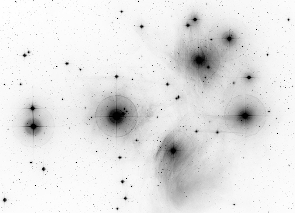
\includegraphics[width = 0.3\tw]{m45.pdf}
    \caption{Рассеянное звёздное скопление M45 (негатив)}
\end{wrapfigure}
\term{Рассеянное звёздное скопление}~--- слабо связанная группа из сотен или тысяч звёзд, сформировавшихся из одного гигантского \imp{молекулярного облака} в одно время, как следствие, имеющих один возраст. Причиной формирования рассеянного звёздного скопления могут служить ударные волны от близких сверхновых, гравитационные взаимодействия внутри облака или столкновение с другим облаком. B силу природы своего образования рассеянные звёздные скопления встречаются  только в тонком диске Галактики, где происходят процессы звёздообразования. Их типичный диаметр~--- несколько парсек.

\begin{figure}[h!]
    \begin{subcaptionblock}{0.48\tw}
        \centering
        \tikzsetnextfilename{hr-m45}
        \begin{tikzpicture}
            \begin{axis}[
                height = 4.5cm,
                width  = 1.05\tw,
                xlabel = {$B-V$},
                ylabel = {$M_V$},
                ymax   = 8.0,
                ymin   = -2.0,
                y dir  = reverse,
                xmax   = 1.5,
                xmin   = -0.25
            ]
                \addplot+[only marks, mark = o, mark options={scale=0.2, black}] table[x=B-V, y=M_V]{data/hr-M45.txt};
            \end{axis}
        \end{tikzpicture}
        \caption{M45 (Плеяды)}
        \label{pic:hr-m45}
    \end{subcaptionblock}
    \hfill
    \begin{subcaptionblock}{0.48\tw}
        \centering
        \tikzsetnextfilename{hr-m67}
        \begin{tikzpicture}
            \begin{axis}[
                height = 4.5cm,
                width  = 1.05\tw,
                xlabel = {$B-V$},
                ylabel = {$M_V$},
                ymax   = 10.0,
                ymin   = 0.0,
                y dir  = reverse,
                xmax   = 1.5,
                xmin   = 0.25
            ]
                \addplot+[only marks, mark = o, mark options={scale=0.2, black}] table[x=B-V, y=M_V]{data/hr-M67.txt};
            \end{axis}
        \end{tikzpicture}
        \caption{M67}
        \label{pic:hr-m67}
    \end{subcaptionblock}
    \caption{Диаграммы Герцшпрунга--Рассела рассеянных звёздных скоплений}
\end{figure}

Рассеянные скопления молоды: из-за слабого гравитационного взаимодействия между звёздами они быстро разрушаются. Поэтому они показывают нам, как происходит эволюция звёзд первые несколько сотен миллионов лет. Только очень тяжелые звёзды из этих скоплений успевают сойти с главной последовательности. И направиться по диаграмме Герцшпрунга--Рассела в область красных гигантов. Таким образом, диаграммы рассеянных скоплений показывают, как эволюционируют звезды, более массивные, чем Солнце.

На \picRef{pic:hr-m45} видно, что даже самые яркие звёзды молодого рассеянного звёздного скопления Плеяды все ещё находятся на главной последовательности. В то в время как в старейшем рассеянном звёздном скоплении M67 звёзды с показателем цвета меньше $0.5^m$ уже стали красными гигантами, \lookPicRef{pic:hr-m67}. На диаграмме видна характерная точка поворота в области абсолютной звёздной величины $3^m$\,--\,$4^m$ и $B-V=0.5^m$, что дает оценку на возраст скопления в районе 4~миллиардов лет.
